\chapter{Results}
\label{sec:results}

A reward model is only as useful as the policies it can train. Offline metrics ask how well it scores trajectories it is handed, but a foundation reward model is meant to be deployed, and in deployment it is queried by an optimizing policy on that policy's own rollouts. That is the setting we care about most, and, as this chapter shows, it is also the one that separates the models most sharply. We build toward it in stages. We first run lightweight comparisons to settle the training recipe, then evaluate the resulting models offline on both in-distribution and out-of-distribution data, and finally use them as the reward signal for downstream reinforcement learning. The central result is a gap between the two regimes, strong offline scores that do not carry over on-policy, and much of the chapter is spent measuring that gap and explaining where it comes from. Throughout, the findings are tied back to the four research questions of the introduction, whether failure data improves the discrimination of success from failure (RQ1), whether an in-context demonstration improves the model's judgment (RQ2), whether an asymmetric loss tames overconfidence and makes the reward harder to exploit (RQ3), and whether offline gains transfer to downstream reinforcement learning (RQ4), and each is restated briefly where it is answered. The recipe and offline sections carry most of the evidence for RQ1 and RQ2, and the downstream sections decide RQ3 and RQ4.

\section{Experimental setup}
\label{sec:exp-setup}

\subsection{Models and baselines}

We evaluate the six fine-tuned models of Section~\ref{sec:method-training}, the two backbones, Robometer-4B and Qwen3.5-VL-4B, each trained in three versions that add one contribution at a time: the standard symmetric loss fine-tuned on our failure data, the asymmetric loss in its place, and finally the addition of in-context demonstrations. Our reference point throughout is the off-the-shelf Robometer-4B, the released reward model before any of our training. On the out-of-distribution set described below it reproduces the numbers reported in the Robometer paper, which validates our evaluation setup. Section~\ref{sec:results-lora} settles the loss these six models share before we train them at full scale.

\subsection{Offline evaluation}

Offline we ask two things of a reward model. The first is whether it orders trajectories correctly, ranking a successful attempt above a failed one and a later frame above an earlier one, where the latter case is only for successful trajectories. We measure this with rank accuracy, the fraction of success-failure pairs the reward orders the right way, and with Kendall's $\tau$ between predicted progress and true frame order. The second is whether the success head, the signal a downstream policy actually reads, separates success from failure at the level of a single frame. Here we report the area under the ROC curve (ROC-AUC) and, to account for the (slight) class imbalance, the area under the precision-recall curve (AUPRC). Most importantly, we report the true-positive rate at a strict five-percent false-positive budget ($\mathrm{TPR}@5\%\,\mathrm{FPR}$). To compute it we sweep the decision threshold over the pooled scores of the evaluation split until five percent of failure frames land above it, then report the fraction of success frames clearing that same cut, so the false-positive rate is fixed by construction and the true-positive rate is what the model achieves at that threshold. This represents the practical operating point for downstream reinforcement learning. Because a strictly zero-percent false-positive threshold in high-dimensional domains typically suppresses the true-positive rate to the point of destroying the learning signal, we accept a 5\% margin to capture more genuine successes.

For the progress head we also report class separation as $d' = (\mu_{\mathrm{succ}} - \mu_{\mathrm{fail}})/\sigma$, the distance between the mean success and mean failure score in pooled standard deviations. A reward can rank pairs correctly on average and still overlap the two classes enough for a false positive to slip through at the threshold a policy uses, and $d'$ is what tells the two situations apart. Every metric in this chapter, offline and downstream alike, is oriented so that higher is better.

We compute every offline metric on two splits. The first is in-distribution, a held-out portion of our own re-curated data. The second is out-of-distribution, the held-out-embodiment evaluation set from Robometer, made of real-world robots and scenes that appear in neither model's training. The two splits behave very differently, and the contrast between them is itself one of the chapter's findings.

\subsection{Downstream reinforcement learning}

The deployment test is downstream reinforcement learning. We train image-based policies with IBRL \citep{hu_imitation_2024}
and replace the sparse binary environment reward with the reward model, querying it on the policy's own rollouts. IBRL bootstraps an off-policy actor-critic, here soft actor-critic \citep{haarnoja_soft_2018}, from a behavior-cloning policy trained on the same demonstrations, which it also keeps in the replay buffer alongside the agent's own rollouts. The off-policy nature of the backbone is of specific importance. An off-policy critic is sensitive to the form a dense reward takes, not only its ranking, and it can bootstrap value from a spurious early terminal, the exploit the minimum episode length is there to close. A run is scored by the task success rate of the policy it produces. As a control we run the identical loop with the simulator's ground-truth reward, which bounds what the setup can reach when the reward is perfect and isolates the reward as the variable under test. We consider two common but different training setups with different policy backbones. One learns from sparse, binary rewards that mark task success, read from the success head, and the other from dense, continuous rewards that track task progress, read per step from the progress head. In both we sweep the weighting and threshold that turn the model's output into a scalar reward. We evaluate on three simulated manipulation benchmarks to test varying degrees of distribution shift. MetaWorld \citep{yu_meta-world_2019, mclean_meta-world_2025} serves as an environment where our model holds an advantage, as the baseline was trained on significantly less MetaWorld data. It is held-out in-distribution in the strict sense, since the domain is familiar but the tasks we train on appear in no reward model's training data. LIBERO \citep{liu_libero_2023} is in-distribution for both reward models, held out at the task level only for the baseline, a provenance Section~\ref{sec:results-rl-libero} spells out, while Robomimic \citep{robomimic} tests both models in a strictly out-of-distribution setting. On MetaWorld and Robomimic the policy backbone is IBRL as described above, while on LIBERO we train with the soft actor-critic implementation released with Robometer, so the baseline is evaluated inside its authors' own reinforcement learning loop.

\section{Choosing the training recipe}
\label{sec:results-recipe}

The full fine-tunes commit to two choices ahead of time, the training objective and the frame budget. This section fixes both by experiment, and every section after it evaluates the models that come out.

\subsection{Choosing the loss}
\label{sec:results-lora}

We train LoRA \citep{hu_lora_2022} adapters of rank $32$ on the attention and MLP projections of Robometer-4B, together with the reward heads, on an $18$k-trajectory sample of the corpus, and evaluate every few hundred steps on held-out slices of each source, DROID, Robometer, MetaWorld, and FailSafe. The training sample has a similar success-failure ratio to the full dataset. The deciding metric is rank accuracy, the fraction of success-failure pairs the reward orders correctly, averaged over the four splits, the same aggregate we later use to compare the full fine-tunes. Every evaluation runs twice, with and without an in-context demonstration.

The study compares the two candidates of Section~\ref{sec:method-loss} and the additions built around them. The ordinal CORN loss runs at $c \in \{0, 0.5, 1.5\}$, with its head freshly initialized because four cumulative logits cannot inherit the pretrained ten-bin head, and the reweighted loss at $\lambda = 0.3$ on top of Robometer's own heads. The hyperparameter for the reweighted loss is selected after a set of preliminary experiments, and Appendix~\ref{apx:lambda} reports the sweep against the milder $\lambda = 0.5$. Around this loss, we also test the task-description dropout and the KL anchor of Section~\ref{sec:method-extras}. We train each variant for 7,500 steps, and then compare each variant at its best checkpoint by the aggregate, the checkpoint that would be selected and carried forward in practice. Appendix~\ref{apx:lambda} breaks these aggregates down per split.

\begin{figure}[t]
\centering
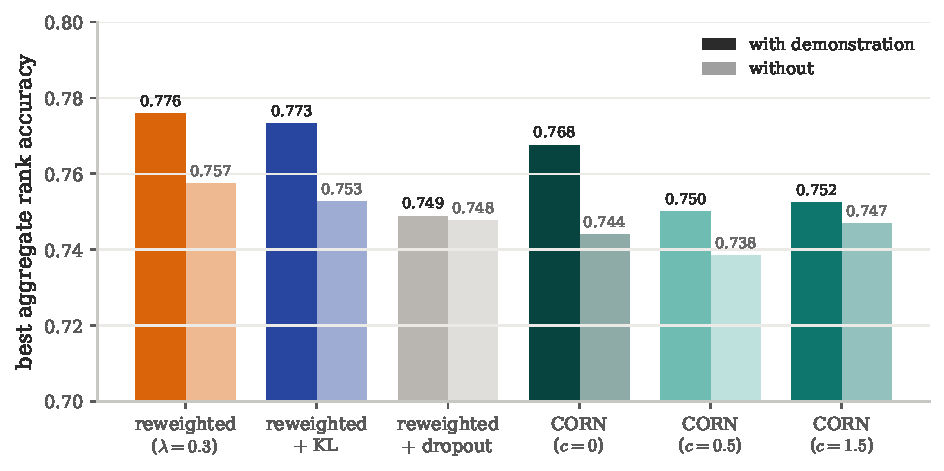
\includegraphics[width=\columnwidth]{media/results/lora_loss_comparison.pdf}
\caption[LoRA loss comparison]{The LoRA loss comparison, each variant at its best checkpoint by the aggregate metric, rank accuracy averaged over the four evaluation splits. The plain reweighted loss posts the highest aggregate of the study, and none of the additions, the ordinal head, task-description dropout, or the KL anchor, exceeds it. The symmetric CORN variant ($c=0$) stopped at three thousand steps, within the window where every variant reaches its peak. Higher is better.}
\label{fig:lora-loss}
\end{figure}

Figure~\ref{fig:lora-loss} compares those best checkpoints. The plain reweighted loss at $\lambda = 0.3$ posts the highest aggregate of the study, $0.776$ with a demonstration attached and $0.757$ without. The CORN family sits below it throughout, and its own ordering actually reveals that the penalization is damaging. The symmetric variant at $c = 0$, which is essentially a standard cross entropy loss, is the best of the three, and pushing the asymmetry up to $c = 0.5$ and $1.5$ makes it slightly worse, so the ordinal formulation pays for its conservatism in ranking quality where the reweighted loss does not. That is the comparison that matters for our purpose, since conservatism is the property we require of the loss, and between the asymmetric variants of each family the reweighted objective leads by a clearer $0.776$ to $0.752$ (CORN with $c=0.5$). Combined with the practical advantage that the reweighted objective resumes directly from Robometer's pretrained heads while the fresh ordinal head must learn its calibration from nothing, we select the reweighted loss for our full fine-tunings.

The two additions of Section~\ref{sec:method-extras} fail despite their well-documented motivation. The KL anchor of Equation~\ref{eq:kl-anchor} at $\lambda_{\mathrm{kl}} = 0.1$ peaks marginally below the plain reweighted run, $0.773$ against $0.776$, and a stronger $\lambda_{\mathrm{kl}} = 0.3$ is no better. We leave it out of the full runs, with the asterisk that the full-scale corpus is far bigger than this $18$k-trajectory sample. Even at a matched success-failure ratio, the anchor's usefulness could look different at that scale. Furthermore, the KL anchor is an expensive addition. Every time a success is seen, the sampled failure's prediction has to be recomputed with the current weights, which means either halving the already-maxed batch size to do this concurrently or paying for it sequentially. Because the anchor adds this overhead without a corresponding gain, we drop it.

The task-description dropout, meant to force the model onto the visual evidence of the demonstration instead of the text, costs about three points of best aggregate instead, $0.749$ against $0.776$, and since it deliberately damages a channel the deployed model relies on, we keep it off.

Gaussian noise on the success labels, drawn per frame at $\sigma = 0.1$ with the endpoints pinned to zero and one, targets a different concern, that the model could learn to tell successes from failures by the shape of the target alone, a smooth ramp against a broken one, and not by content (Section~\ref{sec:method-dataset}). Figure~\ref{fig:label-noise} illustrates the scheme on schematic targets. It neither rescues the CORN head it is paired with nor improves the reweighted loss, and it blurs an otherwise clean training signal, so it too is dropped, the suboptimal outcome Chapter~\ref{sec:methodology} anticipated.

\begin{figure*}[t]
\centering
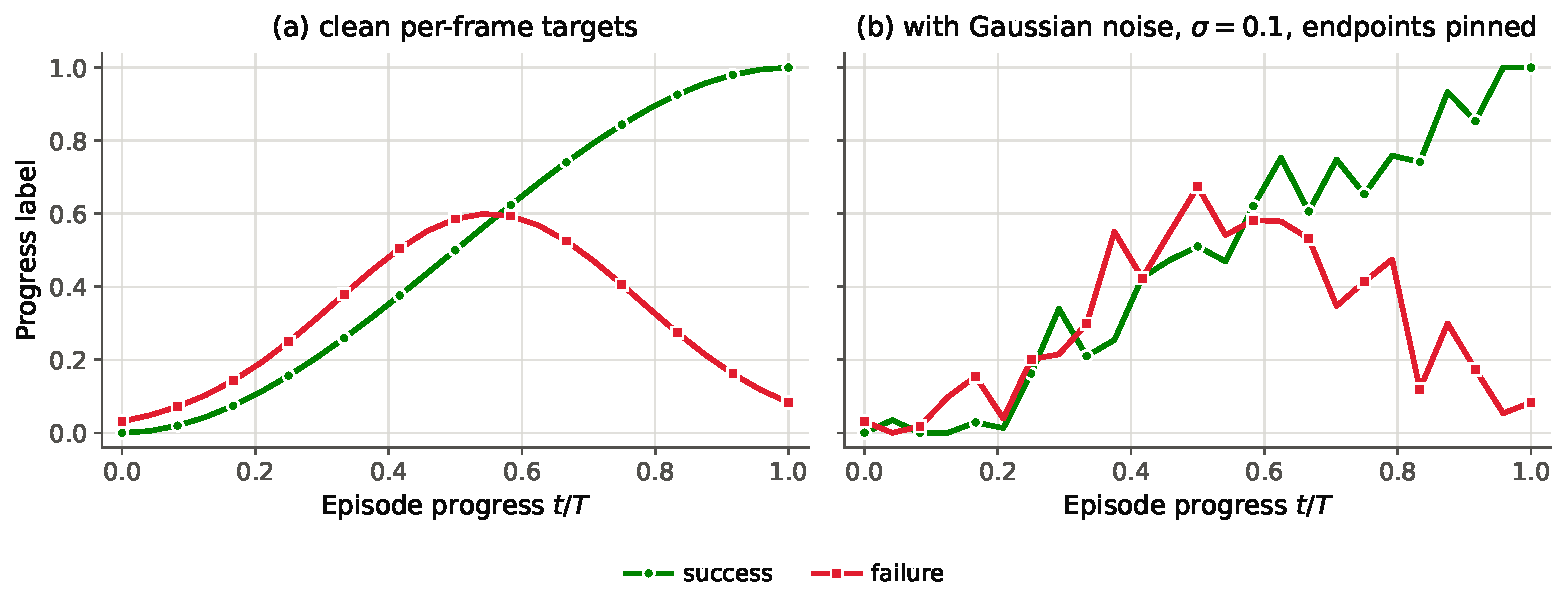
\includegraphics[width=0.92\textwidth]{media/results/label_noise.pdf}
\caption[Gaussian label noise]{The label-noise variant of the recipe study, illustrated on schematic targets. \emph{(a)} Clean per-frame progress targets for a successful and a failed episode, separable by shape alone, a smooth ramp against a broken one. \emph{(b)} The same targets with per-frame Gaussian noise at $\sigma = 0.1$ and the endpoints pinned, which disguises the shape while preserving the labels the heads must learn. The addition neither rescued the ordinal head nor improved the reweighted loss, so it was dropped.}
\label{fig:label-noise}
\end{figure*}


The configuration that emerges is the one Section~\ref{sec:method-training} trains at full scale, the reweighted asymmetric loss with $\lambda = 0.3$ on both heads, no KL anchor, no task-description dropout, and no label noise.

\subsection{Eight or sixteen frames}
\label{sec:results-frames}

Section~\ref{sec:method-arch} doubles Robometer's frame budget from eight to sixteen. We therefore train an eight-frame variant of the full in-context model under an otherwise identical recipe, and compare.

\begin{figure*}[t]
\centering
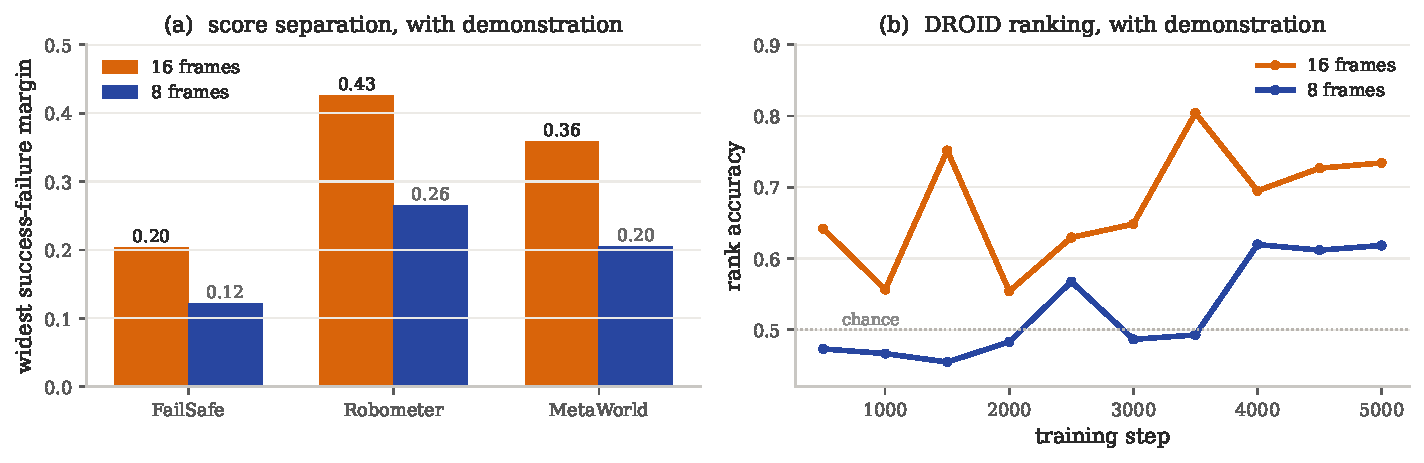
\includegraphics[width=\textwidth]{media/results/frames_8v16.pdf}
\caption[Eight versus sixteen frames]{The frame-budget ablation on the full in-context fine-tune, using the best asymmetric loss formulation. Both panels evaluated with a demonstration attached. \emph{(a)} The widest success-failure margin per split, where a task's margin is the mean score of its successes minus the mean score of its failures. Sixteen frames widen the best margin substantially on all three splits. \emph{(b)} Rank accuracy on DROID over training, where the sixteen-frame model leads at every evaluation. Higher is better in both panels.}
\label{fig:frames}
\end{figure*}

Figure~\ref{fig:frames} depicts the impact of using more frames. With a demonstration attached, sixteen frames widen the best success-failure margin substantially on all three shown splits, $0.12$ to $0.20$ on FailSafe, $0.26$ to $0.43$ on Robometer, and $0.20$ to $0.36$ on MetaWorld, and the mean margin across tasks moves in the same direction. Panel~(b) turns to DROID and to rank accuracy, the share of success-failure pairs the reward orders correctly, where the sixteen-frame model leads at every evaluation and finishes at $0.734$ against $0.620$. DROID is a special case, as it is the only real-world dataset and is significantly more difficult, so the comparison shows that more frames help most exactly where the data is toughest. One reason is more visual information. Another is temporal resolution. The moment that decides a real-world clip's score, a slipping grasp or a dropped object, can fall between two of eight frames and vanish, and with a demonstration attached the benefit compounds, since the demonstration's resolution doubles too. We keep sixteen frames for all six production runs.

\section{Offline reward quality}
\label{sec:results-offline}

Our position throughout this thesis is that downstream reinforcement learning is the evaluation that matters. We still measure offline quality first, for two reasons. It compares our six models and the released baseline on the footing prior work reports, and the gap between what it predicts and what the downstream evaluation later shows is itself one of this chapter's findings. We evaluate on the two splits of Section~\ref{sec:exp-setup}, one held out from our own corpus and therefore held in-distribution, and Robometer's held-out-embodiment set, out of distribution for every model in the table. Every model is scored with and without an in-context demonstration, including the models that never trained with one. Running both isolates the contribution of the demonstration itself, and the control is not empty for the released baseline, whose pretraining included a preference objective that presented two rollouts jointly, so a demonstration alongside the query is not an entirely unfamiliar input and could in principle help it.

\begin{table}[t]
\centering\footnotesize
\caption[Offline ranking, in-distribution]{Offline ranking, in-distribution, by the progress head. Rank accuracy is the fraction of success-failure pairs ordered correctly, $\tau$ is Kendall's correlation with true frame order. Both are reported with and without an in-context demonstration, including for the Qwen3.5 models that never trained with one. Higher is better for both metrics.}
\label{tab:offline-id-rank}
\begin{tabular}{@{}lcccc@{}}
\toprule
 & \multicolumn{2}{c}{no demonstration} & \multicolumn{2}{c}{with demonstration} \\
Model & rank-acc & $\tau$ & rank-acc & $\tau$ \\
\midrule
Robometer-4B (released) & 0.611 & 0.437 & 0.625 & 0.397 \\
RoboRef-ICL & 0.821 & \textbf{0.707} & \textbf{0.896} & \textbf{0.818} \\
RoboRef-Asym & \textbf{0.846} & 0.692 & 0.731 & 0.741 \\
RoboRef-Std & 0.771 & 0.591 & 0.747 & 0.672 \\
Qwen3.5-FT (asym $+$ ICL) & 0.834 & 0.669 & 0.842 & 0.676 \\
Qwen3.5-FT (asym) & 0.743 & 0.412 & 0.731 & 0.550 \\
Qwen3.5-FT (standard) & 0.813 & 0.617 & 0.693 & 0.398 \\
\bottomrule
\end{tabular}
\end{table}

\begin{table}[t]
\centering\footnotesize
\caption[Offline success detection, in-distribution]{Offline success detection, in-distribution. The success head is the signal downstream reinforcement learning reads, so its precision-recall area, its true-positive rate at a five-percent false-positive budget, and its ROC area are the numbers that matter most; $d'$ is the class separation of the progress head. Higher is better throughout.}
\label{tab:offline-id-succ}
\begin{tabular}{@{}lcccc@{}}
\toprule
Model & AUPRC & TPR@5\%FPR & ROC-AUC & $d'$ \\
\midrule
Robometer-4B (released) & 0.67 & 0.24 & 0.67 & 0.42 \\
RoboRef-ICL & \textbf{0.91} & \textbf{0.55} & \textbf{0.88} & \textbf{1.54} \\
RoboRef-Asym & 0.89 & 0.54 & \textbf{0.88} & 1.31 \\
RoboRef-Std & 0.88 & 0.51 & 0.87 & 1.08 \\
Qwen3.5-FT (asym $+$ ICL) & 0.69 & 0.23 & 0.69 & 0.54 \\
Qwen3.5-FT (asym) & 0.65 & 0.15 & 0.64 & 0.27 \\
Qwen3.5-FT (standard) & 0.64 & 0.14 & 0.65 & 0.32 \\
\bottomrule
\end{tabular}
\end{table}

In distribution, the RoboRef fine-tunes win across the board (Tables~\ref{tab:offline-id-rank} and~\ref{tab:offline-id-succ}). The operating point we care about most is the strict five-percent false-positive budget, where the reward must catch successes without paying out on failures, and there the fine-tuned models recover $0.51$ to $0.55$ of true successes against the baseline's $0.24$. We weight this metric most heavily because even our fine-tuned models remain overconfident despite the asymmetric loss, so the operating point that matters is the one that separates the classes without letting enough false positives through to poison an RL policy. The demonstration columns of Table~\ref{tab:offline-id-rank} also settle the control from the setup. The models that never trained with a demonstration mostly lose rank accuracy when one is attached, while the released baseline's small gain, $0.611$ to $0.625$, is consistent with its preference-era exposure. Its preference head taught it to read two trajectories in one input, a skill our non-ICL fine-tunes inherited but then partly lost, since they drop that head and never see a second trajectory again, ordinary catastrophic forgetting under fine-tuning. Either way, none of this approaches the jump the model trained with demonstrations shows. The benefit of in-context learning is earned in training, not granted by the input.

RoboRef-Std, which changes nothing of Robometer's recipe but the training data, isolates what the failure data alone contribute, and the contribution is large. Rank accuracy rises from $0.611$ to $0.771$ and the TPR at the same FPR threshold is more than double, going from $0.24$ to $0.51$. Adding the asymmetric loss on top improves every metric further, and adding the demonstration improves $d'$ most of all, $1.08 \to 1.31 \to 1.54$ across the three RoboRef fine-tunes. That progression matters because $d'$ is a very significant metric. A reward can rank the average success above the average failure and still let a policy find the overlap between the two distributions given an unstable standard deviation, so a demonstration that widens $d'$ is directly shrinking the false-positive rate available for a policy to exploit.

The headline result is that RoboRef-ICL is the best performing model overall, leading on $d'$ and on almost every other metric, and beating the baseline by more than $27$ percentage points in rank accuracy when a demonstration is given. It is also the most robust model without one, posting the best Kendall's $\tau$ of the field, evidence that training with a coin flip over whether to attach a demonstration, so the model works in both regimes, pays off. The one metric where it is not the best is rank accuracy without a demonstration, and only by a small margin. Finally, the suboptimal performance of the baseline is surprising considering the strong offline reward metrics reported in Robometer's paper. RBM-1M contains 100 demonstrations of MetaWorld tasks, far smaller than our own MetaWorld set. However, it still means that during training it has seen MetaWorld examples, making this inferior performance noteworthy.

The Qwen3.5 models, trained from cold heads without Robometer's reward pretraining, are close to the baseline's results on the success head and below their RoboRef counterparts on most metrics, most clearly in Table~\ref{tab:offline-id-succ}. The Qwen3.5-FT model trained with in-context learning is the standout among them, reaching $0.834$ rank accuracy without a demonstration, yet its success head (Table~\ref{tab:offline-id-succ}) is markedly weaker. Whether this gap reflects the base model or the missing reward pretraining is not something our experiments can separate. A Qwen3.5 model pretrained on Robometer's own recipe before our fine-tuning would answer this question, but that is beyond our compute budget, so the rest of this thesis centers on the stronger RoboRef models.

\begin{figure*}[h]
\centering
\begin{minipage}{\textwidth}
  \centering
  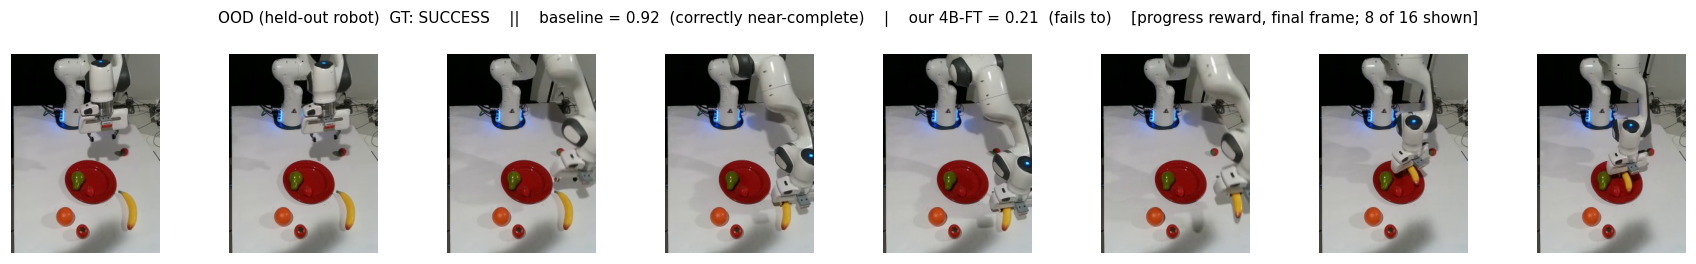
\includegraphics[width=0.93\textwidth]{media/results/ood_example.png}\\[2pt]
  {\footnotesize (a) out of distribution, the task ``Put banana on plate'' on a held-out robot, annotated a success in the evaluation set itself. Baseline $0.92$, ours $0.21$.}\\[6pt]
  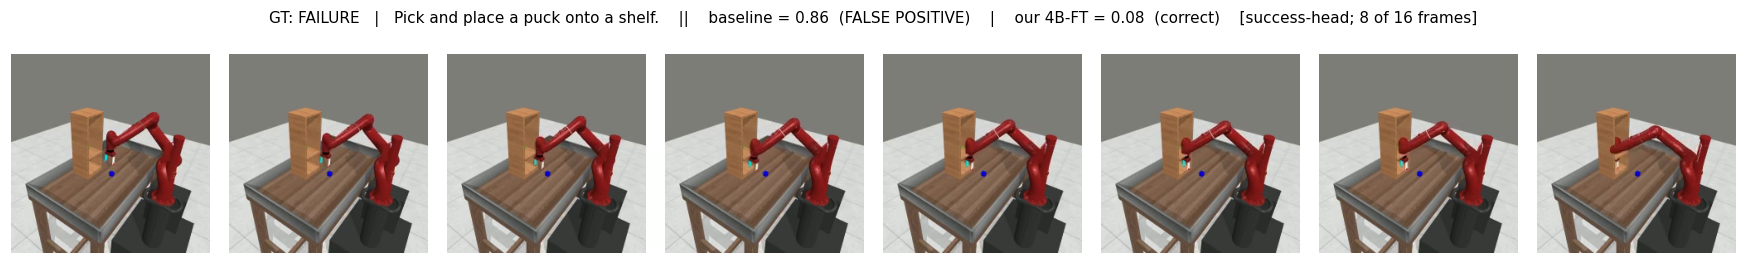
\includegraphics[width=0.93\textwidth]{media/results/id_fp_example.png}\\[2pt]
  {\footnotesize (b) in distribution, a failed attempt to pick up a puck and place it onto a shelf. Baseline $0.86$, a false positive; ours $0.08$.}
\end{minipage}
\caption[Offline trade-off on two clips]{The offline trade-off on two single clips, progress and success read on the final frames with the standard expectation readout for both models. \emph{(a)} Out of distribution the released baseline recognizes a completion our fine-tune appears to miss; the low value is largely the expectation readout compressing the fine-tune's bimodal output (Appendix~\ref{apx:condmean}). \emph{(b)} In distribution the baseline pays out on a failure our fine-tune correctly rejects.}
\label{fig:offline-qual}
\end{figure*}

Figure~\ref{fig:offline-qual} compares the baseline against our headline model, RoboRef-ICL. The upper plot reads the progress head on a successful out-of-distribution trajectory. The lower plot reads the success head on a failed in-distribution one. Two things stand out. First, the baseline scores both clips high, $0.92$ for the success and $0.86$ for the failure, which reveals its sensitivity to false positives. A genuine failure should not sit this high on the 0-1 scale, as well as this close to a genuine success, even if some threshold between $0.92$ and $0.86$ would technically separate them. Second, our model does separate the two with a cleaner margin, but notice that its own output is much smaller even on the success. The compression is not the model's judgment but an artifact of the standard readout on our model's bimodal output, which we return to shortly.



\begin{table}[h]
\centering\footnotesize
\caption[Offline reward metric evaluation, out of distribution]{Offline reward metric evaluation, out of distribution, on a $571$-episode held-out-robot set spanning six robots none of the models saw in training. The first two columns read the success head, its ROC area and its true-positive rate at a five-percent false-positive budget. The last two read the progress head, decoded as the mean conditioned on the model having moved off its lowest bin, since the fine-tuned heads' distributions are bimodal on this set (Appendix~\ref{apx:condmean}). Higher is better throughout.}
\label{tab:offline-ood}
\setlength{\tabcolsep}{3.5pt}
\begin{tabular}{@{}lcccc@{}}
\toprule
 & \multicolumn{2}{c}{success head} & \multicolumn{2}{c}{progress head} \\
\cmidrule(lr){2-3}\cmidrule(lr){4-5}
Model & AUC & TPR@5\% & rank-acc & $\tau$ \\
\midrule
Robometer-4B (released) & \textbf{0.86} & 0.38 & \textbf{0.81} & \textbf{0.63} \\
RoboRef-ICL & 0.84 & \textbf{0.40} & 0.75 & 0.50 \\
RoboRef-Asym & 0.79 & 0.28 & \textbf{0.81} & 0.58 \\
RoboRef-Std & 0.76 & 0.16 & 0.76 & 0.50 \\
Qwen3.5-FT (asym $+$ ICL) & 0.69 & 0.24 & 0.70 & 0.14 \\
Qwen3.5-FT (asym) & 0.66 & 0.16 & 0.64 & 0.28 \\
Qwen3.5-FT (standard) & 0.66 & 0.16 & 0.59 & 0.23 \\
\bottomrule
\end{tabular}
\end{table}

Subsequently, we compare our RoboRef variants directly with a released OOD dataset from Robometer on Table~\ref{tab:offline-ood}. Robometer's baseline leads three of the four columns, but only by a few points on rank accuracy and Kendall's $\tau$, and at the operating point we care about most, the true-positive rate at a five-percent false-positive budget, our headline model, RoboRef-ICL, actually edges past it, $0.40$ against $0.38$. Also, the Qwen3.5 variants demonstrate a disappointing performance in comparison to the RoboRef models, which reinforces our decision to continue only with the RoboRef models for the rest of the chapter.


One computational note applies to the progress columns that we briefly mentioned before. The fine-tuned heads produce bimodal bin distributions on this set, and the released readout, the expectation over the bins, collapses under that shape, so we decode every model with the conditional mean instead, the same expectation taken after the lowest bin is dropped and the rest renormalized. The change leaves the baseline's numbers untouched, its distributions are unimodal, and it lifts the asymmetric model's Kendall's $\tau$ from $0.16$ to the $0.58$ reported in the table. Appendix~\ref{apx:condmean} explains the readout, shows the distributions behind it, and answers why the in-distribution tables do not need it.

\begin{figure*}[t]
\centering
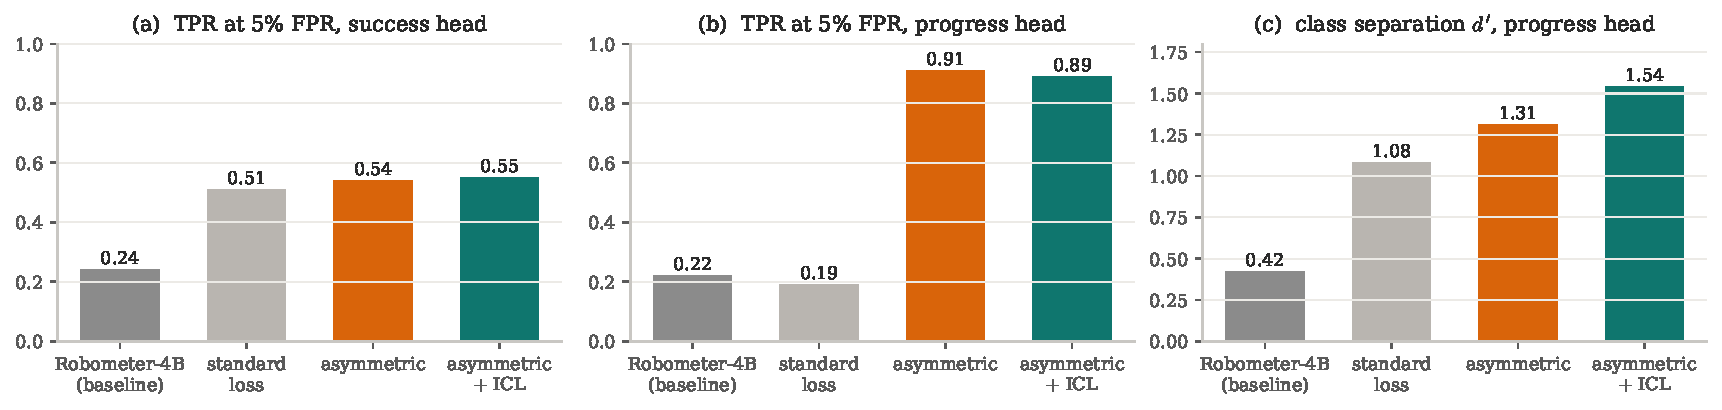
\includegraphics[width=\textwidth]{media/results/asym_offline.pdf}
\caption[What the asymmetric loss buys offline]{What the asymmetric loss buys on the in-distribution evaluation, isolated by comparing the three RoboRef fine-tunes against the released baseline. \emph{(a)} True-positive rate of the success head at a five-percent false-positive budget. \emph{(b)} The same operating point on the progress head. \emph{(c)} Class separation $d'$ between success and failure scores. The standard-loss fine-tune improves the success head but leaves the progress head unusable at a strict false-positive budget; the asymmetric loss delivers on both heads and separates the classes most cleanly. Higher is better in every panel.}
\label{fig:asym-offline}
\end{figure*}

\begin{figure*}[t]
\centering
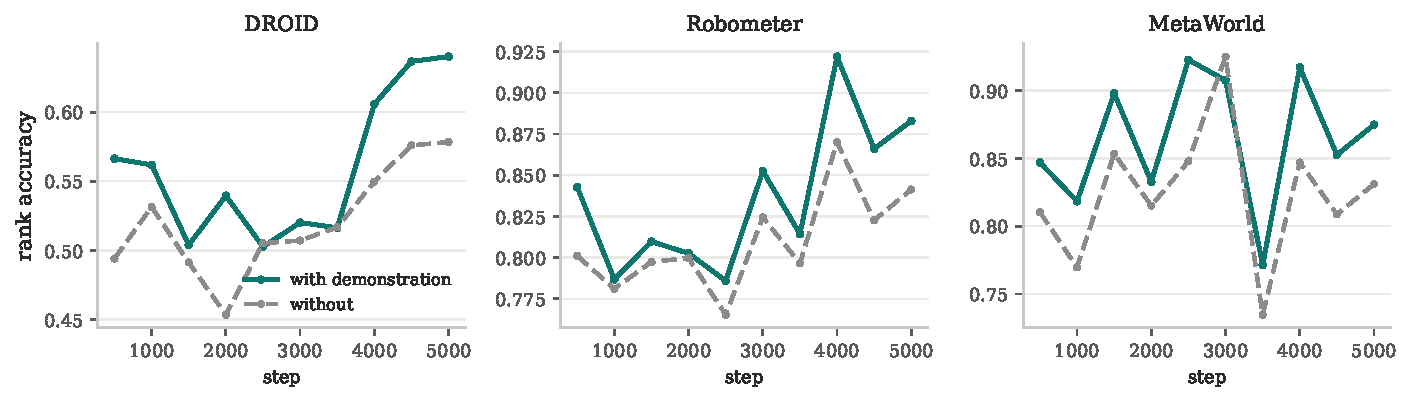
\includegraphics[width=\textwidth]{media/results/icl_convergence.pdf}
\caption[In-context demonstrations over training]{Rank accuracy over training for the full in-context model, evaluated with and without a demonstration, per evaluation split. The demonstration-conditioned evaluation leads on every split for essentially all of training, with the largest margin, still growing at the end, on DROID, the one real-world split. Higher is better.}
\label{fig:icl-convergence}
\end{figure*}

Set beside the in-distribution tables, there is a sharp contrast. There the RoboRef models lead every metric by a wide margin. Here, the baseline leads most of them and RoboRef-Std, already the weakest of the three RoboRef models in distribution, is again the weakest here, trailing on every column but rank accuracy. The reason is the ordinary cost of fine-tuning on a narrower, arm-focused corpus. Sharpening the model's judgment on the data it was trained on trades away some of the released model's broader visual coverage. Moreover, an interesting note is that since this dataset is OOD it should depict the robustness of Robometer-4B in various datasets. However, as we reported before, its performance in our in-distribution dataset, composed of MetaWorld, DROID, FailSafe, and Robometer, where all datasets are also in-distribution for the baseline, shows that the baseline is not as robust as the OOD dataset was suggesting. The asymmetric loss and the in-context demonstration still perform strongly here despite that cost, which is why the model that carries both, our headline model, matches or beats the baseline at the one operating point that matters most for downstream use, the strict-budget true-positive rate.


For the asymmetric loss, the cleanest comparison is between the three RoboRef fine-tunes, identical in everything but the objective, and Figure~\ref{fig:asym-offline} shows that it delivers by far the best class separation. On the success head, panel~(a), the true-positive rate at a five-percent false-positive budget rises from $0.51$ under the standard loss to $0.54$ and $0.55$ under the asymmetric ones, more than doubling the baseline's $0.24$. The progress head, panel~(b), is where the loss matters most, since the standard-loss variant recovers only $0.19$ of successes at that budget, no better than the released baseline, while the asymmetric models recover about $0.9$, and $d'$, panel~(c), rises from $1.08$ to $1.31$ without demonstrations and $1.54$ with them. The loss compresses the score scale yet overlaps the classes less, which is exactly the conservative shape it was designed to produce, and out of distribution the asymmetric variants are still the stronger pair, clearly ahead of the standard-loss fine-tune on the success head and on the constrained FPR operating point (Table~\ref{tab:offline-ood}). Although RQ3, the overconfidence question, mainly targets the RL experiments, the offline reward metric results depict that an asymmetric loss leads to better class separation and stronger true-positive rates at certain thresholds, which is one of our surprising, but positive, findings of this thesis.


\section{What the failure data and the demonstrations contribute}
\label{sec:results-icl}

RQ1 asks whether supervising the reward model on curated failure trajectories improves its ability to discriminate success from failure. In distribution the answer is unambiguous. As Section~\ref{sec:results-offline} showed, changing nothing about Robometer's recipe but the training data lifts rank accuracy by sixteen points and doubles the strict-budget true-positive rate, gains from the failure data alone. Out of distribution the same model trails the baseline on every column of Table~\ref{tab:offline-ood}, but the set itself is a coarse, $571$-episode policy-ranking benchmark, only $166$ of which are labeled outright failures, not the dense failure supervision our own corpus provides, so it is a weak test of what the failure data can do. We do not extend the offline evaluation further to chase a better one, since the test that matters most, downstream reinforcement learning, is next.

The comparison above isolates the data while keeping the loss fixed. One extra experiment closes the loop from the other side, keeping the data fixed and changing only the loss. We continued training the released model on its own corpus, with our added sources removed, under the same recipe as RoboRef-Asym, the same step budget, and the same checkpoint selection rule, so the only ingredient of ours it receives is the asymmetric loss. Table~\ref{tab:offline-abl} scores it on both evaluation splits. 

The loss alone moves almost nothing, and this is clearest on the in-distribution split. Trained on Robometer's own corpus, the asymmetric loss lifts rank accuracy from the baseline's $0.61$ to $0.64$ and its Kendall's $\tau$ actually drops, while the identical recipe on our data reaches $0.85$ and $0.69$, a gap of more than twenty points that the objective alone clearly cannot produce. Out of distribution the picture repeats. The ablation stays within noise of the baseline on the success-head area and on both progress columns, and at the strict false-positive budget it is clearly worse, because the loss reshapes the calibration without failure examples to separate the classes with. Robometer's corpus feeds the asymmetric terms very little, its failures enter training only as preference pairs, a few hundred batches over the whole run. Its progress head also keeps the unimodal shape of the released model, so the bimodal output our fine-tunes develop, the one Appendix~\ref{apx:condmean} studies, traces back to the failure data as well and not to the objective.

Up to this point the in-distribution gains could still be credited to the different loss function, since the asymmetric variants beat the standard one on every table. With both directions now tested, our data under their loss gains a lot and their data under our loss gains almost nothing, the credit falls on the failure data itself. The loss is an amplifier, and without our data it has nothing to amplify.

\begin{table}[h]
\centering\footnotesize
\caption[Loss-versus-data ablation]{The loss-versus-data ablation on both evaluation splits. The middle row trains the released model on its own corpus with our asymmetric loss and nothing else of ours. Its in-distribution scores come from the training pipeline's held-out evaluation at the selected checkpoint, computed on the same data sources as Table~\ref{tab:offline-id-rank}; the out-of-distribution columns use the held-out-robot set of Table~\ref{tab:offline-ood}. Its progress head stays unimodal, so the standard expectation readout applies to it, as it does to the baseline. Higher is better throughout.}
\label{tab:offline-abl}
\setlength{\tabcolsep}{2.5pt}
\begin{tabular}{@{}lcc@{\hskip 8pt}cccc@{}}
\toprule
 & \multicolumn{2}{c}{in-distribution} & \multicolumn{4}{c}{out of distribution} \\
\cmidrule(lr){2-3}\cmidrule(l){4-7}
 & \multicolumn{2}{c}{progress head} & \multicolumn{2}{c}{success head} & \multicolumn{2}{c}{progress head} \\
Model & rank-acc & $\tau$ & AUC & TPR@5\% & rank-acc & $\tau$ \\
\midrule
Robometer-4B (released) & 0.61 & 0.44 & \textbf{0.86} & \textbf{0.38} & \textbf{0.81} & \textbf{0.63} \\
$+$ our loss, their data & 0.64 & 0.36 & \textbf{0.86} & 0.16 & 0.80 & 0.60 \\
RoboRef-Asym (our data) & \textbf{0.85} & \textbf{0.69} & 0.79 & 0.28 & \textbf{0.81} & 0.58 \\
\bottomrule
\end{tabular}
\end{table}

Moreover, the in-context demonstration is the clearest single win in this chapter. With one attached, RoboRef-ICL reaches $0.896$ rank accuracy and $0.818$ Kendall's $\tau$ in distribution, more than $27$ percentage points above the baseline and the best number on almost every column of both in-distribution tables. Figure~\ref{fig:icl-convergence} scores RoboRef-ICL twice at every evaluation, with and without the demonstration attached. The demonstration wins on every split at essentially every stage of training, and by the largest margin on DROID, where the gap is still growing when training ends. The effect predates the full fine-tunes too, since every variant of the LoRA study already gained from a demonstration (Appendix~\ref{apx:lambda}). This mirrors the result of Figure~\ref{fig:frames} which suggested that the number of frames matters for harder tasks. Real-world clips pair cluttered scenes with terse task descriptions, so they benefit most from any additional information the input carries, whether more frames or a demonstration. The demonstration doubles the input length and with it the cost of a step, a price worth paying for a model meant to score real robots. In terms of RQ2, the demonstrations improve the model's judgment throughout, and most where the data is hardest.

The asymmetric loss is the other consistent winner. Across every offline table in this chapter, in-distribution ranking, in-distribution success detection, and out of distribution, the asymmetric variants beat the standard-loss fine-tune, with the class separation of Figure~\ref{fig:asym-offline} the clearest sign of it. The $d'$ of $1.31$ that the loss reaches without a demonstration matters on its own, since it shows the objective earns strong class separation with no help from in-context learning. We expect this conservatism to matter most once the reward is queried by an optimizing policy.

Taken together, the failure data supplies the signal, the demonstrations unlock it on real-world data, and the asymmetric loss turns it into a conservative, well-separated reward. Whether that survives an optimizing policy is the question the rest of the chapter takes up.

\section{Downstream reinforcement learning}
\label{sec:results-rl}

Everything so far has scored the reward models on data they were handed. The deployment test reverses that, letting an optimizing policy query the reward on its own rollouts, and it is the setting the whole chapter has been pointing toward. We evaluate on the three simulated benchmarks of Section~\ref{sec:exp-setup}, MetaWorld, LIBERO, and Robomimic. Because all three share the same reward configurations, we set those out first and refer back to them in each benchmark.

\subsection{Reward configurations}
\label{sec:results-rl-config}

The principle behind these configurations is that every reward model is run as its own authors intend, given its preferred inputs and its native reward form, instead of being forced into a single common protocol. Where the configurations differ they favour the baselines, not our models. The baselines are handed their richest inputs, a goal image and several camera views for one of them (RoboDopamine), a dense per-frame signal for two (RoboDopamine and LRM), and in one case a larger backbone than any of our own models (LRM, at eight billion parameters against our four), while our models are given nothing they were not already designed to use. Whatever advantage our models show is therefore a conservative one, measured against baselines running at their best, which is a harder test for us. Table~\ref{tab:rl-config} summarizes the settings, and the paragraphs below give the detail that the later sections refer back to.

\begin{table*}[t]
\centering\small
\setlength{\tabcolsep}{6pt}
\caption[Reward-model deployment configurations]{How each reward model is queried during reinforcement learning, shared across all three benchmarks. Our models act as success detectors that terminate an episode on detection. The baselines keep their native reward forms and preferred inputs, the configurations under which their authors report results, which favours them.}
\label{tab:rl-config}
\begin{tabular}{@{}lllll@{}}
\toprule
Model & Signal & Protocol & Conditioning & Size \\
\midrule
RoboRef & success head & autonomous, ends on detection & threshold, min length; ICL adds a demo & 4B \\
Robometer-4B & success head or dense progress & best form per benchmark & threshold, min length & 4B \\
RoboReward & rubric $1$--$5$ & full episode, reward at end & zero-shot & 4B \\
RoboDopamine & dense progress & full episode, dense & goal image, multiple views & 4B \\
LRM & dense progress & full episode, dense & initial-frame anchor & 8B \\
\bottomrule
\end{tabular}
\end{table*}

Our own models, RoboRef-Asym and RoboRef-ICL, are deployed the same way in all three benchmarks. They read the success head alone, as a sparse reward in the autonomous protocol of Section~\ref{sec:exp-setup}, and never the progress head, with the single exception of the LIBERO regime study that Section~\ref{sec:results-rl-libero} motivates separately. Every frame the policy produces is scored, and the moment the success probability crosses the model's threshold the episode is declared solved, terminating with the reward paid at that step alone. This is the ordinary way a reward model is used as a success detector, and it makes the reward's task unforgiving, since a single false fire both ends the episode prematurely and pays out a reward the policy never earned. The model has to be right about success and, just as importantly, silent about everything else.

Turning a continuous probability into that fire-or-not decision needs a threshold. A threshold is not particular to our reward; it is what any continuous score requires to act as a detector, and the models in this comparison emit their scores on plainly different scales, so a single shared cut would flatter one and starve another. We therefore calibrate one threshold per model, with an identical procedure for every model in the figure, ours and the baselines alike. On a small set of oracle rollouts collected once and kept out of training, we select the operating point that recovers the most true successes under a strict false-positive budget, the same conservative operating point we argued for offline. Because the recipe is shared, the calibration cannot be what separates the models, and whatever gap remains belongs to the reward itself. 

\begin{figure*}[t]
\centering
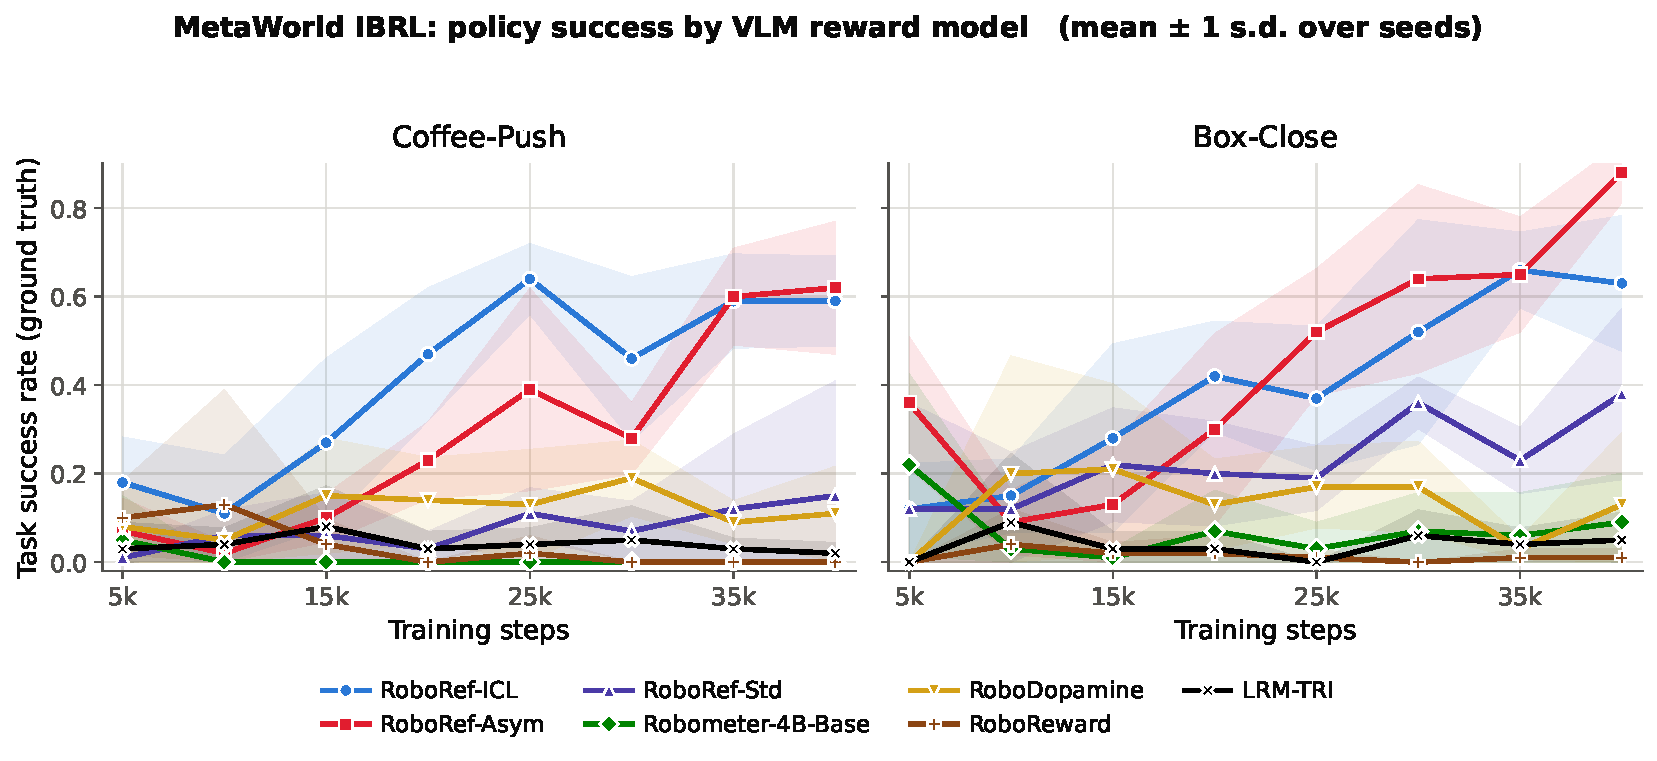
\includegraphics[width=\textwidth]{media/results/metaworld_rl.pdf}
\caption[MetaWorld downstream reinforcement learning]{MetaWorld downstream reinforcement learning, two held-out tasks absent from every reward model's training data, five seeds per reward, mean ground-truth success over training with a one standard deviation band. Success is true task success, measured where the reward model is never queried, not the reward the policy reads. Each reward runs in its Table~\ref{tab:rl-config} configuration, which favours the baselines, so the comparison is conservative for our models. Legend: RoboRef-ICL, RoboRef-Asym, and RoboRef-Std are our fine-tunes with asymmetric-plus-ICL, asymmetric, and standard loss, and Robometer-4B-Base is the released baseline. Only the two asymmetric fine-tunes train a competent policy. Every other reward model ends far behind.}
\label{fig:mw-rl}
\end{figure*}

This calibration does read ground truth, a small set of labeled rollouts, which is a real cost to an otherwise zero-shot deployment, so it matters that the procedure is a convenience and not a requirement. We observe that among the different simulators and different tasks, all thresholds separating successes and failures can be found between 0.75 and 0.9, for both our deployment models. Specifically, RoboRef-Asym varies between 0.75 and 0.85 and RoboRef-ICL between 0.8 and 0.9. The behavior of the policy is a good indication of whether the threshold is too high or too low. A low threshold leads to false positives, failures recognized as successes, which lead to early terminations and flat ground truth evaluations. A high threshold leads to full episodes and minimal signal, as it means that no episodes, either successful or not, manage to surpass the threshold. Thus, this calibration is a technique to quickly find a good threshold for our model ablations and the other baseline VLM reward models, but is not strictly necessary to get a working model.

Furthermore, we fix a minimum episode length per task. IBRL rests on off-policy actor-critic updates, and those methods are susceptible to an early-training exploit, where a policy learns to provoke a spurious success in an episode's first few steps, before the task is physically solvable, collect the terminal reward, and reset. We saw this failure across the reward models, ours and the baselines alike. To overcome it and avoid a flat, dead policy, we ignore any success signal that fires before the episode reaches the minimum. As a simple heuristic, we set the minimum to the length of a demonstration of the given task, drawn from the set the IBRL policy is pretrained on. This encodes a plain physical prior, that nothing is solved faster than an expert solves it, so any earlier fire is spurious by construction. We experiment with minimums between $0.8$ of the demonstration length and the full length, the results in the next sections use the best configuration, and we return to this design choice in Chapter~\ref{sec:discussion}.


Alongside our own models, RoboRef-Asym and RoboRef-ICL, we run three published vision-language reward models, each in the configuration its authors intend. RoboReward \citep{roboreward} scores a whole rollout on a one-to-five rubric and returns a single reward at the episode's end. RoboDopamine \citep{robodopamine} and LRM \citep{TRI-reward-model} emit dense per-frame progress, which we deliver as a shaped increment, each given the input its design expects, a goal image and multiple camera views for the former and an initial-frame anchor for the latter. The comparison also carries the released Robometer-4B from before any of our training, together with our standard-loss fine-tuned ablation, so that within each benchmark a single figure isolates the released model, the failure data, the loss, and the demonstrations in turn. The released baseline is a special case among these, since its paper deploys the progress head as a dense reward while its success head also works as a sparse detector. We do not force one choice on it and instead report its stronger form on each benchmark, naming the form used in each section.

\subsection{MetaWorld}
\label{sec:results-rl-mw}

We begin with MetaWorld, the one environment where our model holds a clear data advantage. That advantage is one of domain, not of memorized tasks, since the two tasks we train on appear in no reward model's training data. We train image-based IBRL policies on these two held-out tasks, Coffee-Push and Box-Close, with five random seeds per reward model, our models reading the success head as a sparse reward under the protocol of Section~\ref{sec:results-rl-config}, and score each seed by the true success rate of the policy it produces, measured in a separate clean evaluation where the reward model is never queried. The curves of Figure~\ref{fig:mw-rl} therefore report ground-truth success, not the model's own reward. The minimum episode length of Section~\ref{sec:results-rl-config} sits at twenty-four steps on Coffee-Push and forty-five on Box-Close, exactly 80\% of the sampled demonstration length.

Figure~\ref{fig:mw-rl} is the widest separation in the thesis. Only RoboRef-Asym and RoboRef-ICL train a competent policy on either task. RoboRef-Asym reaches a mean success of $0.50$ on Coffee-Push and $0.72$ on Box-Close, and RoboRef-ICL holds the same band, $0.55$ and $0.60$. Nothing else comes close. The three published baselines stay under $0.13$ throughout, and the released Robometer-4B, strong enough offline to reproduce the numbers reported in its own paper, moves the policy almost nowhere under either of its forms, $0.00$ on Coffee-Push and $0.07$ on Box-Close at its better one, the sparse detector.

The curve that shows training on MetaWorld data is not the sole factor of this victory is RoboRef-Std, our own standard-loss fine-tune. It sees exactly our failure data and differs from the asymmetric models in the objective alone, and offline it looked the part, recovering half of all successes at the strict false-positive budget (Table~\ref{tab:offline-id-succ}). Under an optimizing policy it comes apart, $0.11$ on Coffee-Push and $0.32$ on Box-Close, well short of the asymmetric fine-tunes trained on the same trajectories. This is the disconnect the chapter has been circling, made concrete on a single pair of curves. Our hypothesis for it is explicit. A fixed test set measures how often a reward is right on average, while an optimizing policy hunts for the specific states where it is wrong, so a model with strong average metrics but exploitable errors, here the false positives the standard loss leaves standing, ranks and detects well offline yet is pulled apart on-policy. The whole distance between the standard and asymmetric fine-tunes is the loss, and it is precisely the distance the conservatism of the asymmetric objective was designed to cover. What read offline as a modest edge in class separation, a $d'$ of $1.08$ against $1.31$ (Table~\ref{tab:offline-id-succ}), is on-policy the line between a reward a policy exploits and one it cannot. This shows plainly what the asymmetric loss does. It does not make the reward more accurate on average; it makes the reward hard to exploit, and being hard to exploit, not offline accuracy, is what decides whether a policy can be trained.

Our hypothesis is that reward hacking is the key factor behind the failed policy learning of every baseline in the figure. Appendix~\ref{apx:mw-reward} traces where it hides by plotting the reward each policy actually received during training. In short, the released Robometer-4B pays the policy the most reward of any model on Coffee-Push while its true success rate stays at zero, the signature of farmed false positives, and the asymmetric fine-tunes pay a smaller reward that climbs together with genuine success. The appendix also verifies that the shared calibration and minimum episode length are not what separates the models, so the advantage sits in the reward itself.

\subsection{LIBERO}
\label{sec:results-rl-libero}

\begin{figure*}[p]
\centering
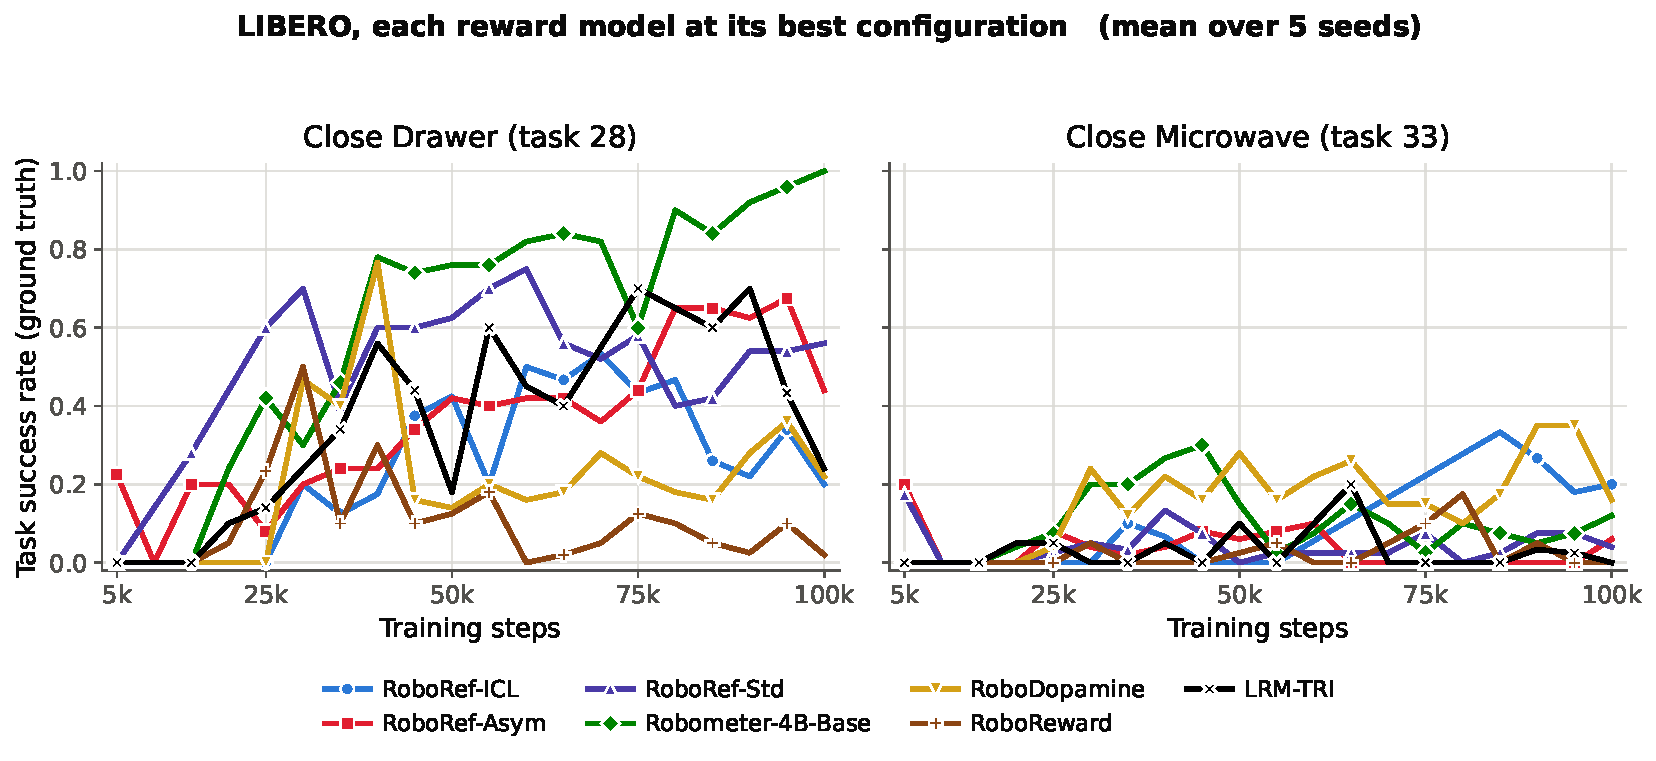
\includegraphics[width=\textwidth]{media/results/libero_rl.pdf}
\captionof{figure}[LIBERO downstream reinforcement learning]{LIBERO downstream reinforcement learning on Close-Drawer and Close-Microwave, five seeds per reward model, mean ground-truth success over training. The tasks are held out from the released baseline's training data though not from our fine-tunes'. Each baseline runs in its Table~\ref{tab:rl-config} configuration, our models in the sparse success-head protocol, and the released Robometer-4B is additionally granted its own preferred form, a dense progress reward with no termination. Under that form the baseline reaches perfect success on Close-Drawer, its strongest result on any benchmark. On Close-Microwave no reward model trains a competent policy.}
\label{fig:libero-rl}
\vspace{14pt}

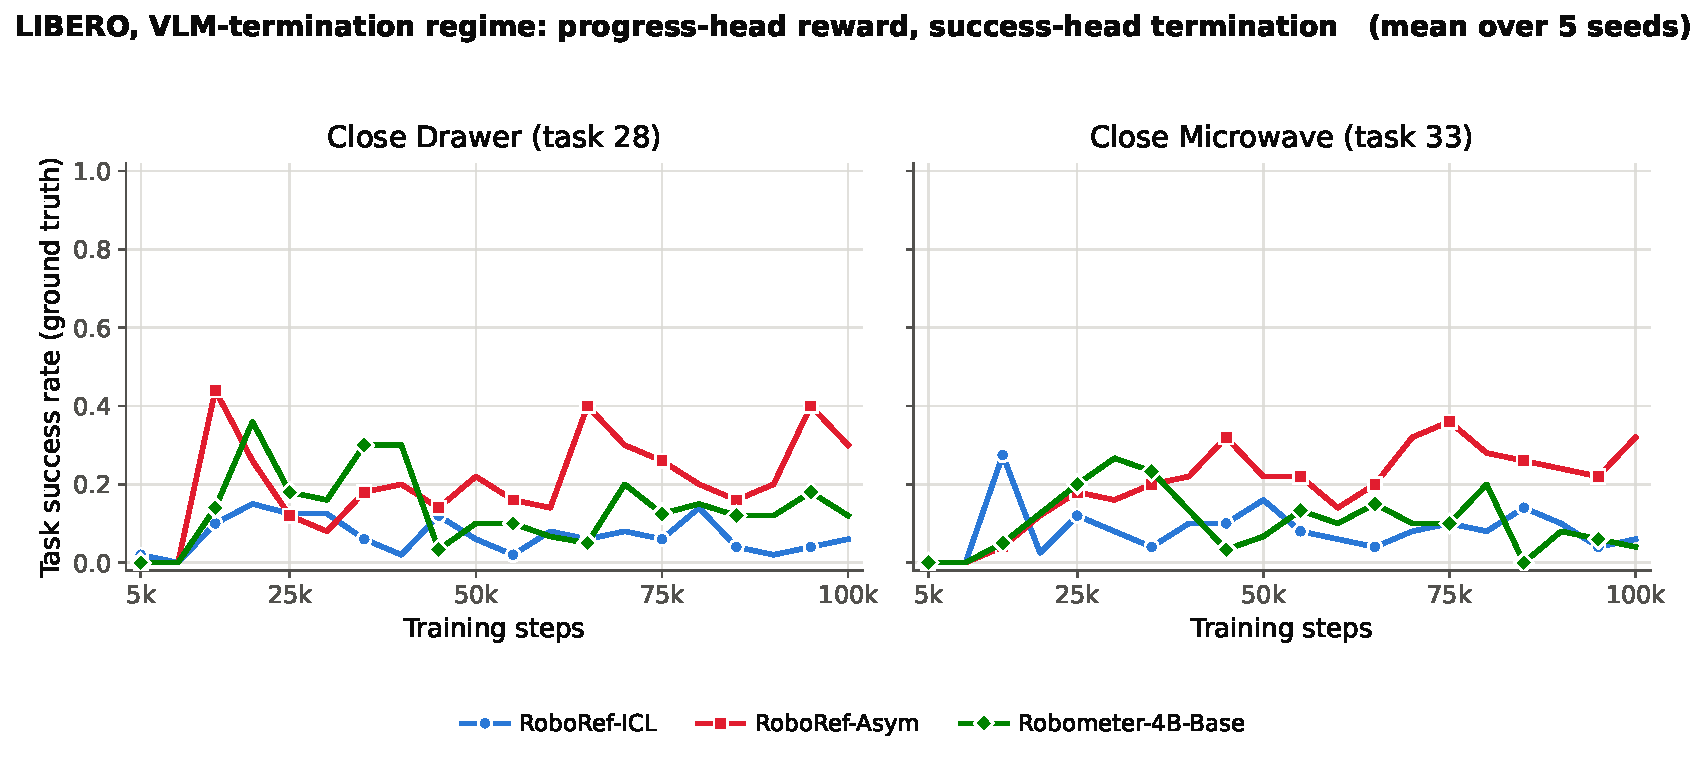
\includegraphics[width=\textwidth]{media/results/libero_termination_rl.pdf}
\caption[LIBERO under the progress-head deployment regime]{The progress heads compared under Robometer's own deployment regime, a dense progress reward with success-head termination, five seeds per model. RoboRef-Asym holds the upper hand on both tasks, as it does on MetaWorld, but no model trains either task well, with every curve peaking below $0.5$.}
\label{fig:libero-termination}
\end{figure*}



LIBERO is the benchmark Robometer itself reports downstream results on, so it is the one place a direct comparison against the released model on its own ground is possible. One property of the setup should be stated before any curve is read. LIBERO-90 is part of Robometer's released training corpus, so our fine-tunes, trained on our re-curation of that corpus, have seen this benchmark during training, while the released Robometer-4B checkpoint predates its inclusion and has not. Its training corpus does include the other LIBERO suites, so the benchmark is still in-distribution for the baseline as well. The comparison is therefore not entirely fair, and the direction of the unfairness runs in our favour, which frames how the results below should be weighed.

We train on two LIBERO-90 tasks, Close-Drawer and Close-Microwave, five seeds per reward model for one hundred thousand steps, and as everywhere else we score each seed by ground-truth task success measured where the reward model is never queried. The setup of Section~\ref{sec:results-rl-config} carries over with one exception. The released Robometer-4B runs here in the dense progress regime with no termination signal, not the sparse detector form it used on MetaWorld, because the dense form is its best configuration on this benchmark and our success rate figures report each model at its best. Our models run the sparse success-head protocol with per-model calibrated thresholds, $0.85$ and $0.80$ on the two tasks for RoboRef-Asym and $0.86$ for RoboRef-ICL, all inside the range the calibration discussion anticipated. The minimum episode length sits at $80\%$ of the demonstration length, where the demonstrations average two hundred steps.

Figure~\ref{fig:libero-rl} shows the comparison at each model's best configuration. Close-Drawer is the one downstream task in this thesis where the released baseline finishes above our models, which comes as a surprise, since the training data would predict the opposite, our fine-tunes have seen LIBERO-90 and the released checkpoint has not. Under its dense, non-terminating form the baseline climbs for the whole run and ends at perfect success. This is the baseline's best showing on any benchmark, and is very different from the rest of its own record, near zero on MetaWorld under every configuration we tried. Our sparse fine-tunes land in the band below it, RoboRef-Asym around $0.65$ late in training and RoboRef-ICL near $0.5$ at its peak, with RoboRef-Std, LRM, RoboDopamine, and RoboReward moving between transient peaks and slow decay. Close-Microwave resists everyone. No reward model, ours or published, trains a policy past $0.35$, and most are well under it, which makes the task less a ranking of models than a shared ceiling on what these rewards can currently teach.

Then, we add one more comparison. Every downstream result of ours so far, on MetaWorld and on LIBERO, reads the success head, so the progress head, the head Robometer's own paper deploys, has not yet driven a policy anywhere in this thesis. Figure~\ref{fig:libero-termination} runs exactly that comparison, our two deployment models against the released baseline, all three under a dense progress-head reward with success-head termination, the exact deployment regime of the Robometer paper. The reward is the per-step progress value, an episode ends when the success head crosses the model's threshold, and the minimum-length rule above still holds.

\begin{figure*}[t]
\centering
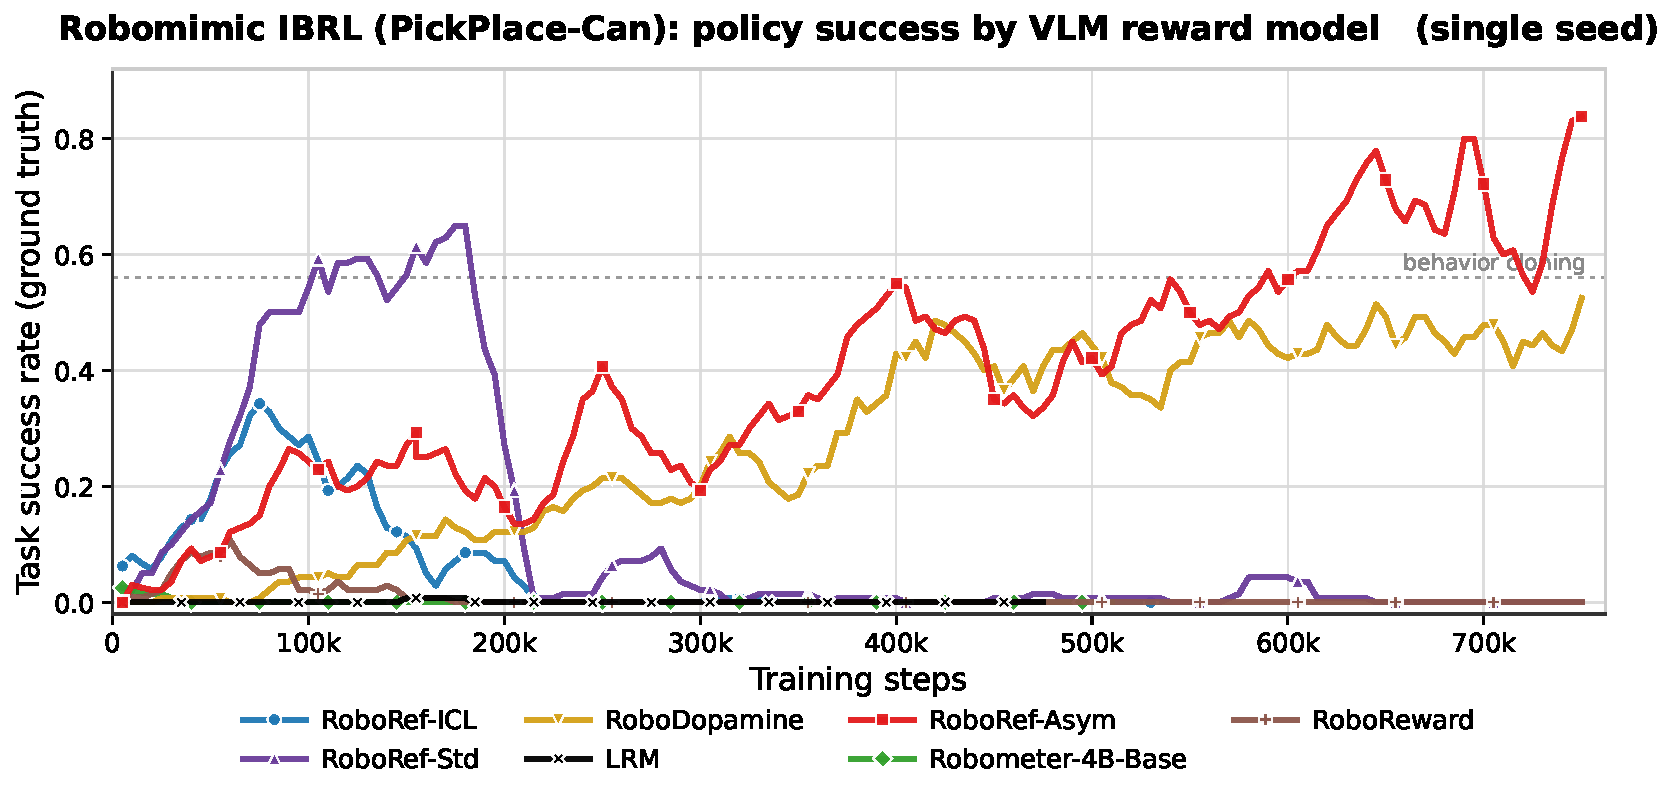
\includegraphics[width=0.72\textwidth]{media/results/robomimic_rl.pdf}
\caption[Robomimic downstream reinforcement learning]{Robomimic downstream reinforcement learning on PickPlace-Can, a domain absent from every reward model's training data, one seed per reward model, smoothed ground-truth success over $750$k training steps. The dashed line marks the behavior-cloning policy that IBRL starts from, at a success rate of $0.56$. Each reward runs in its Table~\ref{tab:rl-config} configuration. RoboRef-Asym is the only reward that ends above the cloning line, at $0.84$ and still climbing; RoboDopamine recovers the demonstrations' competence without exceeding it; RoboRef-Std and RoboRef-ICL rise early and collapse; everything else stays at the floor.}
\label{fig:robomimic-rl}
\end{figure*}

The three models are comparable across both tasks, RoboRef-Asym holds the upper hand for most of training on both, echoing its MetaWorld standing, and the released baseline stays within reach of it, closer than anywhere else in our downstream results. At the same time nothing here approaches the sparse-protocol numbers, every curve on both tasks peaks below $0.5$, and neither task can be called well trained under this regime. 

This result shows two things. First, the released Robometer-4B is weaker than its paper suggests, since in the paper's own configuration it fails to train a good policy on either task. In their figure, however, the model was further trained with LoRA on LIBERO tasks, which apparently was necessary to get good performance. Second, under the regime these models are most naturally built for, a dense reward that leverages the dense labels while the success head closes the episode, none of the models succeeds, ours included.

\subsection{Robomimic}
\label{sec:results-rl-robomimic}

Robomimic is the last benchmark of this evaluation. No reward model in this comparison, ours or the published ones, ever trained on its scenes or its rendering, so every reward is judging a world it has never seen. The task is PickPlace-Can, lifting a can out of one bin and placing it into another. The setup of Section~\ref{sec:results-rl-config} carries over, our models again reading the success head as a sparse reward, with two practical differences. Robomimic steps far more slowly than the other simulators, so a $750$k-step run takes several days and we report a single seed per reward model, spending the compute budget on covering models, not repetitions. And the minimum episode length sits at the full demonstration length of $120$ steps in comparison to the $80\%$ MetaWorld used, because at the lower setting the familiar failure pattern returned, success signals fired before the task was physically solvable and the policies began farming them.

The results can be seen in Figure~\ref{fig:robomimic-rl}. Because IBRL starts from the behavior-cloning policy, the dashed line at $0.56$ is the bar that matters, and any curve that ends above it has learned something the demonstrations alone could not teach. One reward clears it. RoboRef-Asym climbs for essentially the whole run, passes the cloning line for good near $590$k steps, and is still rising at $0.84$ when the budget ends. This is the result we most wanted from this benchmark. On a domain that is fully out of distribution for the reward model, the conservative fine-tune carried an RL policy well past the demonstrations it started from.

Among the baselines, RoboDopamine is the only one that trains a real policy, climbing steadily to $0.53$. It earns the credit for that, and it still ends just below the cloning line, so it recovers the competence already in the demonstrations without moving beyond it. RoboReward and LRM never leave the floor, while Robometer-4B, back in its sparse detector form after its dense LIBERO run, returns to a flat performance like MetaWorld.

In addition, RoboRef-Std is the fastest starter in the figure, above the cloning line within roughly $105$k steps and peaking at $0.65$. Its only differences from the released Robometer-4B, flat at zero for the entire run, are our training data and the dropped preference head, so this early stretch is RQ1, the failure-data question, measured on-policy. The failure supervision alone turns a reward that never moves a policy on this domain into one that drives genuine learning for its first two hundred thousand steps, clearing the cloning line at its peak. 

What the data cannot do alone is hold the gain. The observation comes first. RoboRef-Std falls from its peak to zero in the space of a few evaluations and never returns, and RoboRef-ICL, after an early rise to $0.34$, comes apart at the same point of training. We have no ground-truth count of false positives on Robomimic to prove the mechanism, but the pattern matches the one MetaWorld made visible, a policy that eventually finds false positives the symmetric loss left standing, and the fine-tune trained with the asymmetric objective on the same data is the one that does not collapse. The offline numbers pointed the other way. On the out-of-distribution table, RoboRef-ICL was the best of our fine-tunes at the strict false-positive budget (Table~\ref{tab:offline-ood}), yet on-policy it is RoboRef-Asym that survives. A single seed warrants some caution about the exact numbers, but the margin between a policy at $0.84$ and a field that ends below the cloning line is not the kind noise produces.

\section{What the downstream results add up to}
\label{sec:results-rl-summary}

MetaWorld and Robomimic sit at opposite ends of the distribution shift the reward models face, one a domain where our training data gives us a clear edge, the other a domain nobody trained on. They return the same verdict. The rewards that train competent policies are the asymmetric fine-tunes, RoboRef-Asym everywhere and RoboRef-ICL where the domain is familiar, while the released baseline and the three published reward models either sit silent at the floor or, at best, give back the competence the demonstrations already contained. The division of labor between our contributions is visible in the curves themselves. The failure data supplies the discriminative signal, which is why RoboRef-Std rises on Robomimic where the released model never moves, and the asymmetric loss is what lets a model keep what the data taught it.

LIBERO sits between those two ends and complicates the verdict in an instructive way. It is the one benchmark where the released baseline posts a genuine win, perfect success on Close-Drawer under its dense, non-terminating form, and the one task nobody trains, Close-Microwave, caps every reward model at $0.35$. The regime study of Figure~\ref{fig:libero-termination} supplies the sharper reading. Under the deployment form its own paper reports, dense progress with success-head termination, the released model trains neither task well, and our fine-tunes, while ahead of it there too, do not convert their offline edge into strong policies either. The benchmark that should have been the baseline's home ground ends up showing that the deployment regime, as much as the model, decides what these rewards can teach. The same study is candid about our own models. The progress head remains their least developed part, since it never produced clear downstream gains in any of our experiments, a limitation the next chapter takes up.

Almost none of this was visible offline, and that is the answer to RQ4, which asked whether offline reward-quality gains transfer to downstream reinforcement learning. The released Robometer-4B reproduces the offline numbers of its own paper and never trains a policy. RoboRef-Std matches the asymmetric models on nearly every offline column and collapses in MetaWorld and Robomimic. The out-of-distribution table ranks RoboRef-ICL above RoboRef-Asym at the strict operating point, and on-policy the order flips. Offline evaluation scores a reward on a fixed set of trajectories, but an optimizing policy is not a fixed set; it is a search process that actively hunts for the inputs the reward gets wrong, and it finds them. The one offline quantity that pointed in the right direction was class separation at the conservative operating point, where the asymmetric loss stood out, and even that only hinted at the size of the on-policy gap. Offline reward-quality gains transfer only when they come packaged with conservatism, and when they do not transfer, the mechanism is the one Figure~\ref{fig:mw-reward} makes visible, a policy farming the reward's false positives. The next chapter takes up what this means beyond our own models.
